


\section{Least Squares Estimation}
\begin{frame}
    \frametitle{Least Squares Estimation}

    The most popular estimation methos is least squares, in which we pick
    the coefficients $\Beta = [\beta_0, \beta_1, ..., \beta_p]^T$ to minimize the
    residual sum of squares. For example, find $\beta_0$, $\beta_1$ that minimize

    $$L(\beta_0,\beta_1) = \sum_{i=1}^{n}(Y_i - \E[Y_i])^2 = \sum_{i=1}^{n}(Y_i - (\beta_0+\beta_1x_i))^2$$


    Find the minimal by solving the linear equation system using partial derivatives.

    $$\frac{\delta~L}{\delta\beta_0} = 0~~~\text{and}~~~\frac{\delta~L}{\delta\beta_1} = 0$$

\end{frame}



\begin{frame}
    \frametitle{Least Squares Estimation: Simple linear regression}

    Partial derivatives: Find the minimal by solving the linear equation system
    \small
    $$\frac{\delta~L}{\delta\beta_0} = -2\sum_{i=1}^{n}(Y_i-\beta_0-\beta_1x_i) = 0 
    \Leftrightarrow {\color{red}n\beta_0+\beta_1\sum_{i=1}^{n}x_i=\sum_{i=1}^{n}Y_i}$$

    \small
    $$\frac{\delta~L}{\delta\beta_1} = -2\sum_{i=1}^{n}x_i(Y_i-\beta_0-\beta_1x_i) = 0 
    \Leftrightarrow {\color{red}\beta_0\sum_{i=1}^{n}x_i+\beta_1\sum_{i=1}^{n}x_i^2=\sum_{i=1}^{n}x_{i}Y_i}$$

    $$\beta_0 = \frac{1}{n}\sum_{i=1}^{n}Y_i - \beta_1\frac{1}{n}\sum_{i=1}^{n}x_i\Rightarrow \overline{Y}-\beta_1\overline{x}$$
    
    $$\beta_1 = \frac{\sum_{i=1}^{n}(x_i - \overline{x})(Y_i - \overline{Y})}{\sum_{i=1}^{n}(x_i-\overline{x})^2}$$

\end{frame}



\begin{frame}
    \frametitle{Least Squares Estimation: matrix formulation}

    Find $\beta$ that minimizes $L(\beta) = (Y-X\beta)^T(Y-X\beta)$.
    From partial derivatives, let's expand $L(\beta)$ and use the fact that all terms
    are scale. Remark $(a-b)^2=a^2-2ab+b^2$.

    $$L(\beta) = (Y-X\beta)^T(Y-X\beta) = Y^TY - 2\beta^TX^TY + \beta^TX^TX\beta$$

    $$\frac{\delta~L(\beta)}{\delta\beta} = -2X^TY + 2X^TX\beta$$

    Where the solution must statisfies the normal equation 
    $$X^TX\beta = X^TY \Rightarrow {\color{red}\beta = (X^TX)^{-1}X^TY}$$
\end{frame}


\begin{frame}
    \frametitle{Least Squares Estimation: matrix formulation}
    \begin{figure}
        \centering
        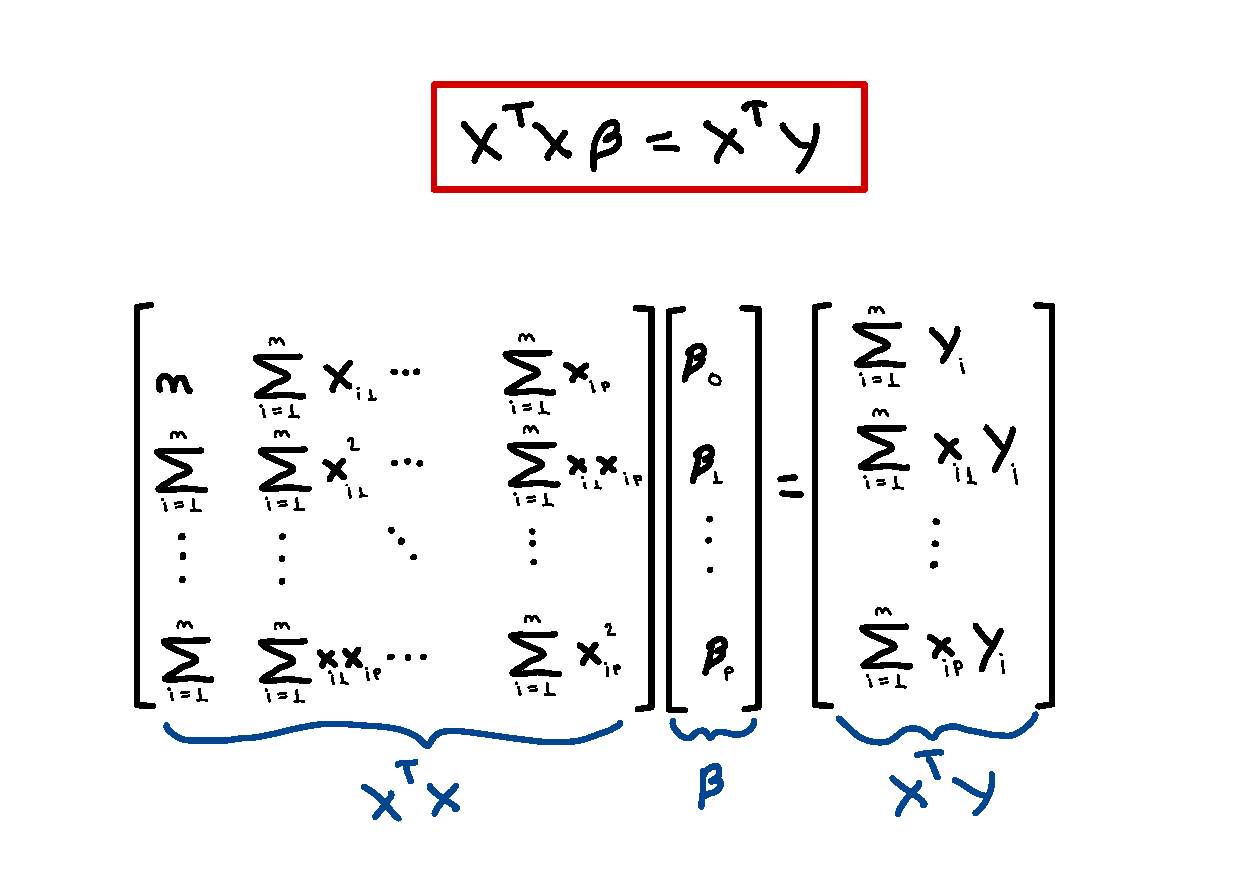
\includegraphics[width=0.95\textwidth]{sections/least_squares_estimation/figures/xxb-xy.pdf}
    \end{figure}
\end{frame}



\begin{frame}
    \frametitle{Least Squares Estimation}

    \begin{itemize}

        \item \textbf{Parameters to estimate}: $\hat{\beta}$ is the solution to the normal equation:
        $$\hat{\beta}=(X^TX)^{-1}X^TY$$
        
        Where (usually) $(X^TX)^{-1}$ is singular and the least squares 
        coefficients $\hat{\beta}$ are not uniquely defined.


        \item \textbf{Predicted values}: fitted line
        $$\hat{Y} = \E[Y_i] = \hat{\beta_0}+\hat{\beta_1}x_{i1}+...+\hat{\beta_{p}}x_{ip} \Rightarrow {\color{red}\hat{Y}=X\hat{\beta}}$$

        \item \textbf{Residuals}: the difference between observations and predictions

        $$e_i = Y_i - \hat{Y_i}s \Rightarrow {\color{red}e = Y - \hat{Y} = Y - X\hat{\beta}}$$
    \end{itemize}

\end{frame}

\begin{frame}
    \frametitle{Least Squares Estimation: Residual variance}

    \begin{itemize}

        \item \textbf{Residual variance}: $s^2$ is an estimate of the variance of the
        error. Remark: a good variance estimator is $\frac{\sum_{i=1}^{n}x_{i}}{f}$, where
        $f$ is the degrees of freedon.

        $$V[\epsilon] = \E[(\epsilon - \overline{\epsilon})^2] = \E[\epsilon^2] = \E[(Y_i-\hat{Y_i})^2] = \frac{\epsilon^T\epsilon}{n-(p+1)}$$

        Where $p+1$ is the total number of $\beta$ parameters (degrees of freedon) in the model and
        $n$ is the number of observations.

    \end{itemize}

\end{frame}


\begin{frame}
    \frametitle{Least Squares Estimation: $\beta$ variance}

    Until here, we assumed that the observations $y_i$ are
    uncorrelated and have contant variance $\sigma^2$ and
    that $x_i$ are fixed (non random).

    \begin{itemize}

        \item \textbf{$\beta$ variance}: The variance-covariance matrix
        of the least squares parameters is derived from 

        $$\hat{\beta} = (X^TX)^{-1}X^Ty$$

        and is given by:

        $$Var(\hat{\beta})=(X^TX)^{-1}\sigma^2$$

        \item Tipically one estimates the variance $\sigma^2$ by:

        $$\hat{\sigma^2}=\frac{1}{N-p-1}\sum_{i=1}^{N}(y_i - \hat{y_i})^2$$

    \end{itemize}

\end{frame}

\begin{frame}
    \frametitle{Least Squares Estimation: $\beta$ variance}
    \begin{figure}
        \centering
        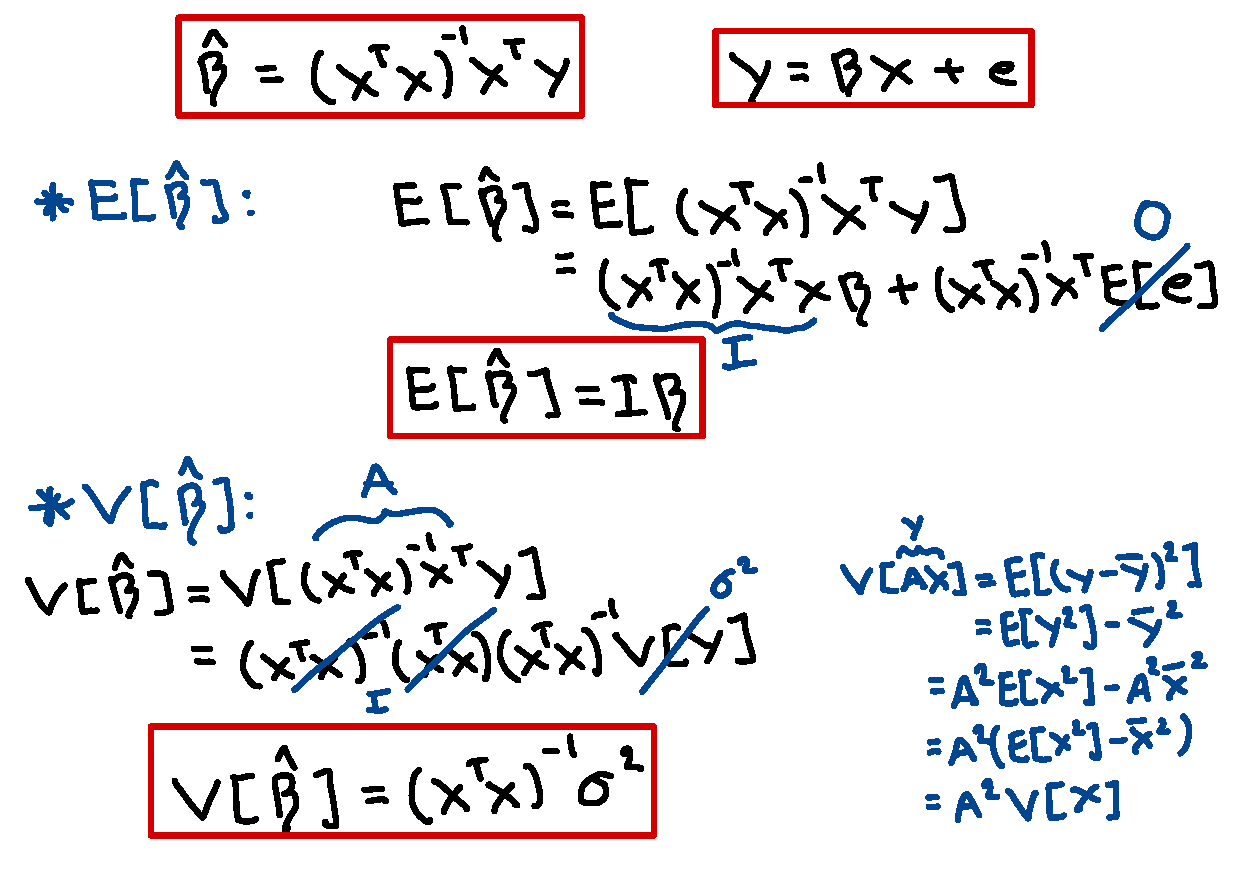
\includegraphics[width=0.95\textwidth]{sections/least_squares_estimation/figures/beta_variance_prove.pdf}
    \end{figure}
\end{frame}


\begin{frame}
    \frametitle{Least Squares Estimation: $\beta$ variance}

    \begin{itemize}

        \item \textbf{The error distribution}: Is a Gaussian random variable with
        $\E[\epsilon]=1$ and $V[\epsilon]=\sigma^2$

        $$\epsilon \approx N(0, \sigma^2)$$

        \item \textbf{The  $\hat{\beta}$ distribution}: Is a Gaussian random variable
        with $\E[\hat{\beta}]=\beta$ and $V[\hat{\beta}]=(X^TX)^{-1}\sigma^2$

        $$\hat{\beta} \approx N(\beta, (X^TX)^{-1}\sigma^2)$$

    \end{itemize}

\end{frame}


\subsection{Multiple Outputs}


\begin{frame}
    \frametitle{Multiple Outputs}
 
    \begin{itemize}
        \item Suppose we have multiple outputs $Y_1, Y_2, ..., Y_k$ that we wish
        to predict from out inputs $X_0, X_1, ..., X_p$. We assume a linear model
        for each output;

        $$Y_k = \beta_{0k} + \sum_{j=1}^{p}X_j\beta_{jk} + \epsilon_k$$

        \item With $N$ training cases we can write the model in matrix notation

        $$Y =  XB + E$$

        Where $Y$ is the $N\timesK$ response matrix, with $y_{ik}$ entries, $X$ is 
        the $N\times(p+1)$ input matrix, $B$ is the $(p+1)\times K$ matrix of 
        parameters and $E$ is the $N\times K$ matrix of erros.
    \end{itemize}

\end{frame}


\begin{frame}
    \frametitle{Multiple Outputs}
 
    \begin{itemize}
        \item A straightforward generalization of the multivariate loss function is

        $$L(B) = \sum_{k=1}^K\sum_{i=1}^N\left(y_{ik} - f_k(x_i)\right)^2$$

        Where $f_k(x_i) = \beta_{ik}x_i$. One for each output column.

        \item In the end, the least squares estimates have exactly the same form as before 

        $$\hat{B} = (X^TX)^{-1}X^TY$$
       
    \end{itemize}

\end{frame}



\subsection{Gauss-Markov Theorem}

\begin{frame}
    \frametitle{Gauss-Markov Theorem}

    One of the most famous results in statistics that the least squares (LS)
    estimates of the parameters $\beta$ have the smallest variance among
    all linear unbiased estimates (such as ridge regression)


    \begin{definition}
    \textbf{Gauss-Markov theorem}: states the result on the mathematical
    optimality of the LS: assuming that the following conditions are met,
    \begin{itemize}
        \item $\E[\epsilon_i]=0$ for all $i = 1,...,n$
        \item $V[\epsilon_i]=\sigma^2$ for all $i = 1,...,n$
        \item $Cov(\epsilon_i,\epsilon_j) = 0$ for $i=j = 1,...,n$ (the error are uncorrelated)
    \end{itemize}


    By Gauss-Markov theorem, LS estimators are \textbf{BLUE} (Best Linear Unbiased
    Estimator), where \textbf{best means minimum variance}.
        
    \end{definition}
\end{frame}



\begin{frame}
    \frametitle{Gauss-Markov Theorem: Proof for BLUE estimator}
    \begin{figure}
        \centering
        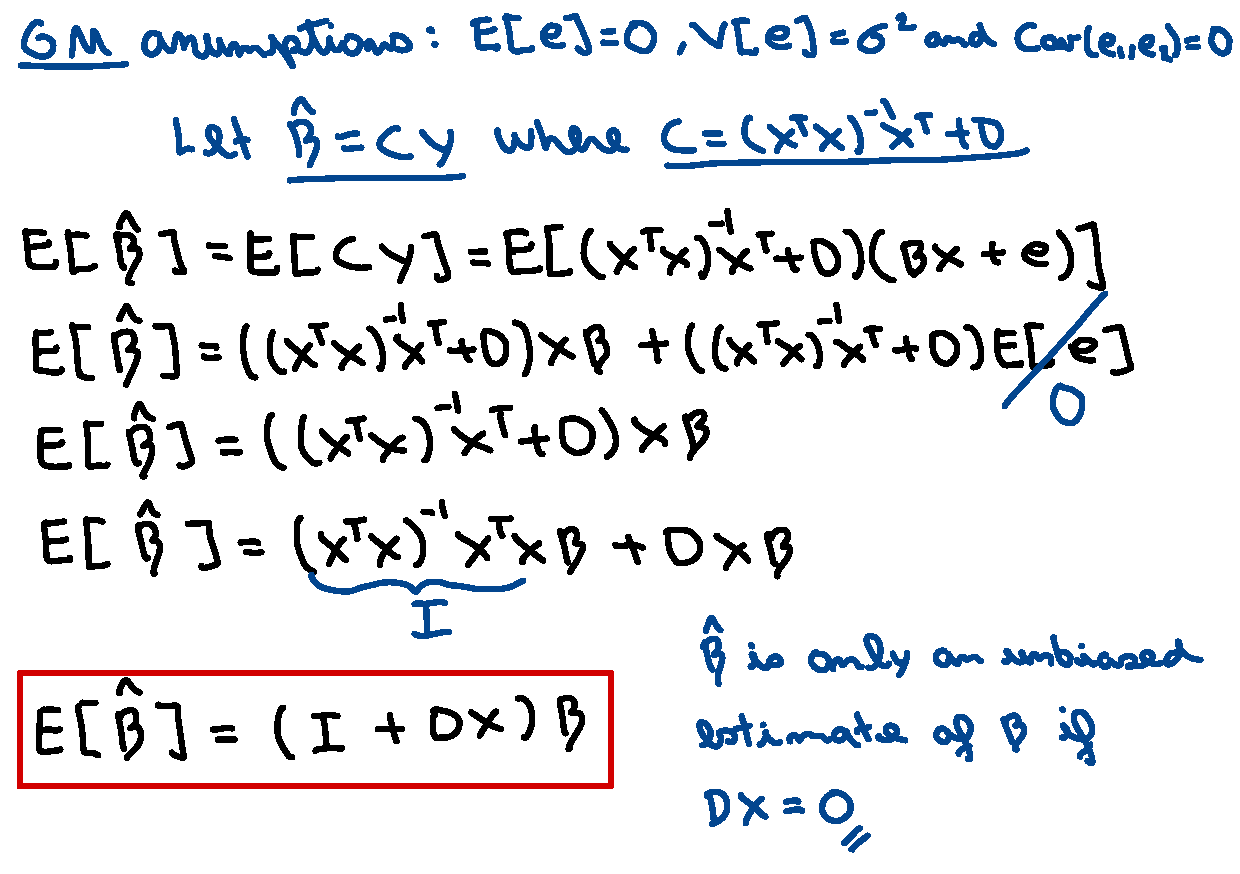
\includegraphics[width=0.95\textwidth]{sections/least_squares_estimation/figures/gm_proof_mean.pdf}
    \end{figure}
\end{frame}



\begin{frame}
    \frametitle{Gauss-Markov Theorem: Proof for BLUE estimator}
    \begin{figure}
        \centering
        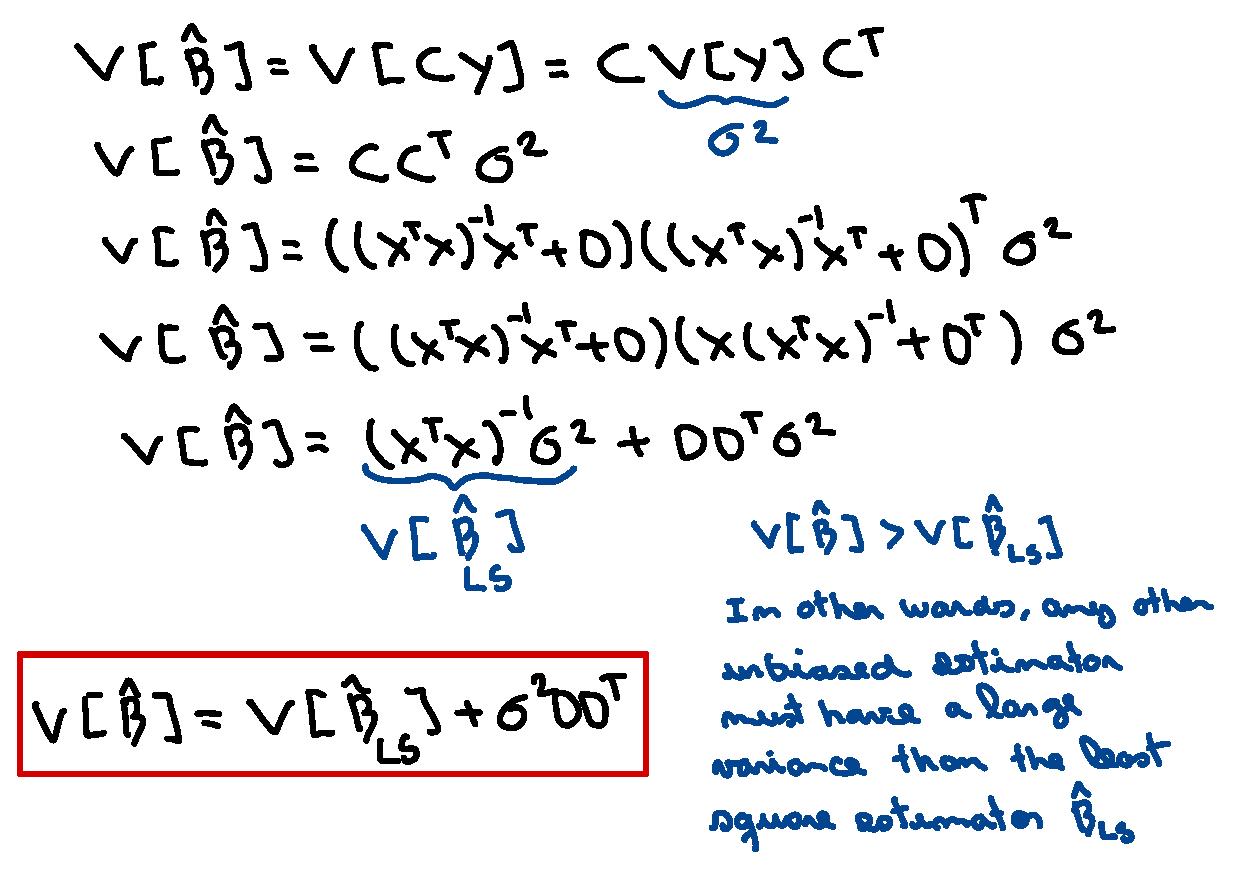
\includegraphics[width=0.95\textwidth]{sections/least_squares_estimation/figures/gm_proof_variance.pdf}
    \end{figure}
\end{frame}

